\newlength{\resultsOverviewModelColWidth}
\newlength{\resultsOverviewCornerHeight}
\newcommand{\resultsOverviewCornerCell}{%
    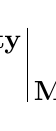
\begin{tikzpicture}[baseline=(current bounding box.center)]
        \path[use as bounding box] (0,0) rectangle (\resultsOverviewModelColWidth,\resultsOverviewCornerHeight);
        \draw[line width=0.4pt] (0,\resultsOverviewCornerHeight) -- (\resultsOverviewModelColWidth,0);
        \node[anchor=north east,inner sep=0pt,xshift=-0.2em,yshift=-0.1ex] at (\resultsOverviewModelColWidth,\resultsOverviewCornerHeight) {\textbf{Capability}};
        \node[anchor=south west,inner sep=0pt,xshift=0.2em,yshift=0.1ex] at (0,0) {\textbf{Model}};
    \end{tikzpicture}%
}

\begin{table*}[t]
    \centering
    \footnotesize
    \caption{\textbf{Cosmos 3 results overview.} Cosmos 3 consistently outperforms specialized open-source baselines across all capabilities. Detailed results can be found in~\cref{sec::results}. In the table, $^\ast$ denotes post-trained Cosmos 3 variants; $\dagger$ denotes closed models; gray-colored cells in each row indicate the model does not possess the corresponding capabilities.}
    \label{tab:results_overview}
    \settowidth{\resultsOverviewModelColWidth}{Lingbot-World-Base (C)}
    \setlength{\resultsOverviewCornerHeight}{2.25\baselineskip}
    \setlength{\tabcolsep}{4pt}
    \resizebox{\textwidth}{!}{%
    \begin{tabular}{l|cccc|cccccc}
        \toprule
        \multirow{2}{*}{\resultsOverviewCornerCell} & \multicolumn{4}{c|}{\textbf{Reasoning}} & \multicolumn{6}{c}{\textbf{Generation}} \\
        \cmidrule(lr){2-5} \cmidrule(lr){6-11}
        & \textbf{General} & \textbf{Robotics} & \textbf{Smart infra.} & \textbf{Driving} & \textbf{Text2Image} & \textbf{Text2Video} & \textbf{Image2Video} & \textbf{Audio} & \textbf{FD: Robot} & \textbf{Policy: Robot} \\
        \midrule
        \rowcolor{rowours}
        \textbf{Cosmos3-Super} & \underline{73.7} & \underline{57.8} & \textbf{62.6} & \textbf{79.3} & \textbf{91.36$^{\ast}$} & \textbf{80.0} & \textbf{82.8} & 7.31 & \textbf{26.0$^{\ast}$} & - \\
        \rowcolor{rowours}
        \textbf{Cosmos3-Nano} & 69.6 & 55.1 & \underline{61.0} & \underline{76.0} & 84.61 & \underline{79.4} & \underline{82.7} & \underline{7.34} & \underline{25.5$^{\ast}$} & \textbf{39.7$^{\ast}$} \\
        \midrule
        Gemini 3.1 Pro$^\dagger$ & \textbf{77.5} & \textbf{58.2} & 58.6 & 47.2 & \cellcolor{black!5} & \cellcolor{black!5} & \cellcolor{black!5} & \cellcolor{black!5} & \cellcolor{black!5} & \cellcolor{black!5} \\
        Qwen3-VL-32B & 72.8 & 52.6 & 56.1 & 40.7 & \cellcolor{black!5} & \cellcolor{black!5} & \cellcolor{black!5} & \cellcolor{black!5} & \cellcolor{black!5} & \cellcolor{black!5} \\
        Qwen3-VL-8B & 68.9 & 48.5 & 52.7 & 46.4 & \cellcolor{black!5} & \cellcolor{black!5} & \cellcolor{black!5} & \cellcolor{black!5} & \cellcolor{black!5} & \cellcolor{black!5} \\
        Gemma-4-31B & 69.8 & 51.0 & 51.3 & 36.6 & \cellcolor{black!5} & \cellcolor{black!5} & \cellcolor{black!5} & \cellcolor{black!5} & \cellcolor{black!5} & \cellcolor{black!5} \\
        Gemma-4-E4B & 53.1 & 39.3 & 29.4 & 26.0 & \cellcolor{black!5} & \cellcolor{black!5} & \cellcolor{black!5} & \cellcolor{black!5} & \cellcolor{black!5} & \cellcolor{black!5} \\
        Gemini 3 Pro Image$^\dagger$ & \cellcolor{black!5} & \cellcolor{black!5} & \cellcolor{black!5} & \cellcolor{black!5} & \underline{90.85} & \cellcolor{black!5} & \cellcolor{black!5} & \cellcolor{black!5} & \cellcolor{black!5} & \cellcolor{black!5} \\
        Qwen-Image-2512 & \cellcolor{black!5} & \cellcolor{black!5} & \cellcolor{black!5} & \cellcolor{black!5} & 84.25 & \cellcolor{black!5} & \cellcolor{black!5} & \cellcolor{black!5} & \cellcolor{black!5} & \cellcolor{black!5} \\
        Veo-3.1$^\dagger$ & \cellcolor{black!5} & \cellcolor{black!5} & \cellcolor{black!5} & \cellcolor{black!5} & \cellcolor{black!5} & 79.1 & 82.6 & \textbf{7.45} & \cellcolor{black!5} & \cellcolor{black!5} \\
        Wan2.2-A14B & \cellcolor{black!5} & \cellcolor{black!5} & \cellcolor{black!5} & \cellcolor{black!5} & \cellcolor{black!5} & 78.0 & 81.3 & \cellcolor{black!5} & \cellcolor{black!5} & \cellcolor{black!5} \\
        Ctrl-World & \cellcolor{black!5} & \cellcolor{black!5} & \cellcolor{black!5} & \cellcolor{black!5} & \cellcolor{black!5} & \cellcolor{black!5} & \cellcolor{black!5} & \cellcolor{black!5} & 23.0 & \cellcolor{black!5} \\
        $\pi_{0.5}$ & \cellcolor{black!5} & \cellcolor{black!5} & \cellcolor{black!5} & \cellcolor{black!5} & \cellcolor{black!5} & \cellcolor{black!5} & \cellcolor{black!5} & \cellcolor{black!5} & \cellcolor{black!5} & \underline{28.1} \\
        \bottomrule
    \end{tabular}%
    }
\end{table*}
